\documentclass[10pt]{article}

\usepackage[a4paper,margin=1in]{geometry}
\usepackage[T1]{fontenc}
\usepackage{lmodern}
\usepackage{amsmath}
\usepackage{graphicx}
\usepackage{booktabs}
\usepackage{caption}
\usepackage{hyperref}
\usepackage{titling}
\usepackage{authblk}
\usepackage[table]{xcolor}
\usepackage{enumitem}
\usepackage{float}

\hypersetup{
  colorlinks=true,
  linkcolor=black,
  citecolor=black,
  urlcolor=blue,
  pdftitle={FreCoS: A Learned Staleness Model for Semantic Caches},
  pdfauthor={Lior Lotan}
}

\captionsetup{font=small,labelfont=bf}

\setlength{\droptitle}{-3em}

\title{\vspace{-1.5em}

\includegraphics[width=6cm]{bgu-logo}\\[1em]
\Large\textbf{FreCoS: A Learned Staleness Model for Semantic Caches}\\[0.3em]
\large A freshness- and cost-aware extension to GPTCache}

\author{Lior Lotan}
\affil{Department of Software and Information Systems Engineering\\
Ben-Gurion University of the Negev}
\date{\today}

\begin{document}

\maketitle

\begin{abstract}
Semantic caches are usually evaluated on hit rate, latency, and at best false-hit rate,
none of which asks whether a hit was still true at the moment it was served. I name that
gap \emph{stale-hit-rate}, the fraction of served hits whose content had already expired,
and extend GPTCache with a per-cluster staleness model used both as a validity gate on
the serve path and as a decay term in eviction. An earlier version of this report
replaced an oracle-cluster, exact-match harness with real embedder-based clustering and
a real semantic index, which reversed the central finding: under real clustering, an
earlier version of the workload's canonical query text differed across clusters only in
two embedded numbers, and a general-purpose embedder could not recover cluster identity
from that (adjusted Rand index 0.02--0.06, barely above chance), so per-cluster
staleness fitting was never actually exercised. This version fixes the diagnosed cause
directly: the canonical text now carries a distinct topic phrase per cluster and a
distinct aspect phrase per answer, raising median adjusted Rand index to 0.42 across a
reduced-scale rerun (3,000 queries, 5 seeds, versus the diagnostic version's 12,000 and
10), and the central claim is restored on a workload that genuinely tests it: learned
per-cluster fitting beats pooling with a large, significant effect, and sits
significantly closer to an unreachable oracle ceiling without fully reaching it. What
else holds: the validity gate cuts stale-hit-rate substantially regardless of clustering
quality, since it applies the same cluster consistently at calibration and serve time;
and a fair test of cost-aware eviction, run for the first time under conditions where
eviction actually occurs, shows FreCoS beating a frequency floor on cost saved with a
large effect, though plain LRU beats FreCoS on both cost saved and stale-hit-rate on
this trace. The text fix does not eliminate false-hit-rate, which remains high (median
0.90--0.91): same-topic, different-aspect queries still score close to the semantic
index's 0.8 cosine match threshold, a more realistic failure mode than the earlier
cross-cluster conflation but still a first-order caveat on every number reported here.
\end{abstract}

\section{Introduction}

\subsection{Motivation}

A semantic cache sits in front of an expensive backend, usually a large language model
call, and serves a stored response when an incoming query lands close enough in
embedding space to one already answered. The promise: skip the call, return the same
answer faster and for free. But ``the same answer'' is a claim about time as well as
similarity, and most semantic caches never check the time part.

This matters most where a language model sits between a user and an answer about content
that changes on its own schedule, for example monitoring how a brand is represented
across AI-generated answers (answer engine optimization). The same style of question
gets asked repeatedly, exactly the workload a semantic cache absorbs, but the facts
behind it do not sit still. A cache that only asks ``have I seen a similar question''
and never ``is that answer still true'' keeps serving a stale answer indefinitely once
written, with no way to tell a correct hit from a wrong one, because stale-hit-rate does
not exist in standard cache evaluation.

Two gaps follow, motivating the two components I add. \textbf{No staleness concept in
the serve path:} a cached answer about a fact with its own expiry schedule is served
indefinitely, with ``found in cache'' silently treated as ``correct.'' \textbf{No cost
term in eviction:} count-based policies such as LRU and LFU treat two entries with
identical access patterns the same way even when one is far more expensive to
regenerate, so a rarely accessed but costly entry can be evicted ahead of a cheap one
merely accessed once more recently.

Industry and research reflect this gap unevenly. Frontier model providers do
exact-prefix key-value caching with a wall-clock TTL and no similarity matching.
Semantic-caching products use a single fixed global threshold with plain TTL or
count-based eviction, with no notion of per-topic staleness. The research literature is
further ahead, proposing cost-aware and staleness-aware eviction formulas, but none
names or measures stale-hit-rate; I compare against that literature, not the weaker
product baseline.

This report makes three contributions. First, stale-hit-rate as a named, measured
metric, and a semantic-index-based harness that exercises it under conditions closer to
a real semantic cache than an oracle-cluster, exact-match one. Second, a diagnosed and
fixed measurement failure: an earlier version of this workload's canonical query
template differed across clusters only in two embedded numbers, which no
general-purpose embedder could use to recover cluster identity (adjusted Rand index
0.02--0.06, at random-assignment level), so per-cluster fitting was never actually
exercised under real clustering in that version. I trace the exact cause, replace the
template with a distinct topic phrase per cluster and a distinct aspect phrase per
answer, and rerun every experiment: with cluster identity now substantially recoverable
(median adjusted Rand index 0.42), learned staleness fitting beats pooling with a
large, significant effect, restoring the report's central per-cluster-learning claim on
a workload that actually tests it. Third, a positive result on cost-aware eviction:
given a fair test under conditions where eviction actually happens, which every earlier
version of this suite failed to arrange, FreCoS's eviction term measurably beats a
frequency floor on cost saved, though it does not beat plain LRU on either metric
tested. Section~2 justifies the baseline, Section~3 describes the design, Section~4
covers the workload and harness, and Section~5 reports seven experiments: one
bracketing run and its two misspecification follow-ups, one five-row ablation, three
parameter sweeps, and one gate-off cost-aware eviction test.

\subsection{Related work}

The closest prior art, and my primary eviction comparator, is Biton and Friedman's work
on semantic-cache eviction~\cite{bitonfriedman2026}. It proves optimal offline
semantic-cache eviction is NP-hard, supplies polynomial-time heuristics, and presents
online policies combining recency, frequency, and locality, evaluated on GPTCache with
released code, part of why I chose GPTCache here. Two findings shape my design: LRU is
weak on semantic workloads, and frequency-based policies are a stronger baseline, which
is why every comparison in this report treats an LFU-class policy, not LRU, as the
floor. FreCoS differs in adding two orthogonal signals, regeneration cost and content
validity over time, and evaluating against a correctness metric, stale-hit-rate, their
setting never defines.

The structurally closest published formula is Cortex's LCFU
policy~\cite{cortex2026}, scoring an entry as log-scaled frequency times cost times
latency times a staleness term, divided by size, with a TTL purge on top. The
difference is narrow: Cortex's staleness term is a static score assigned by a language
model at write time, while FreCoS learns a decay rate per cluster from observed
staleness; Section~\ref{sec:brackets} tests whether that learning does measurable work.
I did not reimplement Cortex's formula, since it relies on remote tool-call latency
metadata with no equivalent here.

Several other lines touch individual pieces without matching the combination:
GDSF~\cite{gdsf2001} ages access recency, not content validity; Category-Aware
caching~\cite{categoryaware2025} assigns load-based, not learned, per-category TTLs
(why I cut a third planned component, calibrated per-cluster thresholds, a lossy special
case of this); FreshCache~\cite{freshcache2026} puts staleness in the serve path as a
probabilistic risk budget rather than a hard gate (future work here);
SCALM~\cite{scalm2024} clusters entries similarly to my k-means step but with no
staleness-aware significance score; MeanCache~\cite{meancache2024} is cost-motivated but
does not target eviction; W-TinyLFU~\cite{tinylfu2015} is admission control, orthogonal
to both my contributions. I considered and rejected vCache~\cite{vcache2025}: its
contribution, per-prompt threshold learning with eviction explicitly out of focus, would
have diluted rather than sharpened the comparison.

\section{Baseline}

\subsection{Why GPTCache}

I extended GPTCache~\cite{gptcache} rather than a more actively maintained semantic
cache, for four reasons. First, its most recent release (v0.1.44, August 2024) is
frozen (maintainers state new integrations have stopped), which is a better
scientific control than a moving target: the baseline measured early in this project is
byte-identical to the one measured at the end. Second, architectural fit, verified by
reading the vendored source directly: every component I touch sits behind a named
interface, so my extension is purely additive (a metadata field via composition, a
serving-path gate in one shared decision helper). FreCoS's eviction policy is the one
exception, added by monkeypatching \texttt{EvictionBase.get()} rather than through any
extension hook, because that factory has none: a hardcoded if/elif chain with no
lookup table a caller could add to. Verified end to end against a real
\texttt{gptcache.manager.data\_manager.SSDataManager} in
\texttt{tests/test\_gptcache\_integration.py}. I never edit vendored code. Third,
GPTCache is the baseline the closest prior art already uses, letting me in principle run
Biton and Friedman's released policy directly, though in practice I substituted a
documented proxy (Section~\ref{sec:ablation}). Fourth, its default embedding backend
runs CPU-deterministically, keeping every run reproducible without a GPU. One trade made
deliberately: GPTCache's README states new contributions are not merged, foreclosing
this course's upstream-adoption bonus.

\subsection{GPTCache's behavior and default eviction policy}

GPTCache serves a cached response when a query is semantically close enough to one
already seen, using a single global cosine threshold (0.8 by default). Its eviction
policies are purely count-based (LRU, LFU, FIFO, random); none reads generation time,
regeneration cost, or retains metadata on an evicted entry, though creation and
last-access timestamps are persisted with no downstream consumer, precisely the gap my
extension repurposes. There is no admission control, and no cost, false-hit, or
staleness tracking anywhere in the built-in reporting layer.

\section{Design}

\subsection{Contribution}

The contribution is one learned artifact with two consumers. FreCoS fits a per-cluster
staleness model and uses it at both ends of the cache's lifecycle: as a hard validity
gate when serving a candidate hit, and as a soft decay term when choosing an eviction
victim. The metric that makes both uses visible is stale-hit-rate: the fraction of
served hits whose content was already invalid when served.

Cluster assignment comes from a fixed, seeded k-means over cached-query embeddings from
GPTCache's default ONNX model, fit once per trace on the calibration split, with every
row assigned to its nearest centroid. This is a change from an earlier version, which
read cluster identity directly off the workload generator's ground truth; every number
in every earlier version of this suite was produced under that oracle-perfect
assignment. Section~\ref{sec:brackets} reports what changes once clustering has to work
from text, the report's central finding. The generator's true label is still recorded on
every row, used only to compute the adjusted Rand index against the learned assignment
(\texttt{cluster\_ari}, reported alongside every bracket-style result), never consumed by
the gate or eviction. Both consumers use the same (possibly wrong) cluster identity and
neither recomputes it independently; I checked directly for disagreement between them in
the ablation (Section~\ref{sec:ablation}) and found none.

For each cluster, a decay rate $\lambda_c$ is fit from observed staleness in a held-out
calibration split, assuming exponential validity decay: $\Pr[\text{still valid after }
\Delta t] = e^{-\lambda_c \Delta t}$. A TTL is derived at confidence level $c$ as
$\text{ttl} = -\ln(c) / \lambda_c$. Three modes produce this table with the same output
shape: \emph{learned} fits each cluster independently by maximum likelihood, falling
back to a pooled rate below thirty observations; \emph{global} pools every cluster
regardless of sample size; \emph{oracle} takes the rate from the generator's ground
truth, an upper bound never available in a real deployment. Table~\ref{tab:params} lists
every tunable parameter, its default, and where its effect is measured.

The validity gate is the first consumer: on a candidate hit, if the entry's age exceeds
its cluster's TTL, it is treated as a miss and the event counts as a stale hit
prevented rather than served. This checks creation time only, never last-access time:
staleness is a property of when an answer was generated, not how recently it was asked
for, so a popular but outdated entry is not treated as fresh just because it is popular.

The eviction value function is the second consumer:

\begin{equation}
\text{value} = \log(2 + \text{freq}) \cdot \log(1 + \kappa \cdot \text{regen\_cost}) \cdot e^{-\lambda_c \cdot \text{age}}
\label{eq:value}
\end{equation}

where $\text{age}$ is from creation time, never last access; $\kappa = 1000$
log-compresses regeneration cost so its heavy tail cannot dominate; the victim is the
lowest-value entry, ties broken by oldest creation then lowest entry id. An earlier
version also divided by \texttt{size\_bytes} to evict larger entries first; that term is
removed, since eviction here runs under an entry-count budget, not a byte budget:
evicting a 10-byte and a 10,000-byte entry both free exactly one slot, so
size-normalization has no budget-economics meaning. This was confirmed empirically at
the highest-eviction-pressure cache-size point in the project's sweep
(\texttt{results/ablation/size\_term\_isolation/}): FreCoS with and without the size term
was statistically indistinguishable on every metric. A byte-budgeted eviction loop,
where size would have real meaning, remains future work.

One detail came from a design mistake a property test caught, not one found by
inspection: my original frequency term, $\log(1+\text{freq})$, is exactly zero for a
never-accessed entry, zeroing the whole product regardless of cost or freshness, so a
freshly written entry would always be evicted next. Appendix A's property test failed
against the literal formula and caught this; I fixed it to $\log(2+\text{freq})$, same
concave shape but strictly positive at zero frequency, applied throughout.

Because the gate already refreshes anything past its TTL, the decay term is not doing
staleness prevention on its own: it is a soft prior among candidates the gate has
already judged fresh. The ablation (Section~\ref{sec:ablation}) tests this directly.

\begin{table}[H]
\centering
\caption{Every tunable parameter, its default, and where its effect is measured in
Section~5. \texttt{Config} ships $c=0.95$; the bracketing and ablation experiments in
Sections~\ref{sec:brackets}--\ref{sec:ablation} run at $c=0.90$, called out wherever
those results appear.}
\label{tab:params}
\begin{tabular}{llll}
\toprule
Parameter & Default & Swept & Measured in \\
\midrule
lambda source (mode) & learned & global, learned, oracle & \ref{sec:brackets} \\
TTL confidence $c$ & 0.95 & 0.80, 0.90, 0.95, 0.99 & \ref{ssec:sweeps} \\
cluster count $K$ & 10 & 5, 10, 20, 50 & \ref{ssec:sweeps} \\
cache size (entries) & 412 (see note) & 5\%--80\% of working set & \ref{ssec:sweeps} \\
$\kappa$ (cost log-compression) & 1000 & not swept & --- \\
calibration fallback threshold & 30 obs.\ & not swept & --- \\
\bottomrule
\end{tabular}
\end{table}

Cache size is 412 entries in the bracketing and ablation experiments; the cache-size
sweep itself spans 5\%--80\% of the working set and identifies 248 entries as the knee
(Section~\ref{ssec:sweeps}). $\kappa$ and the thirty-observation fallback threshold were
fixed at values reasonable at design time and not independently swept.

\section{Experimental setup}

\subsection{Workload}

All experiments run on W1, a deterministic, seeded synthetic workload generator built
for this project. Before other implementation work, I timeboxed a feasibility spike into
a second workload derived from Wikipedia revision history: an automatic
sentence-change rule agreed with hand labels only 40\% of the time against an 80\%
go/no-go bar set in advance (full spike in \texttt{docs/w2-feasibility.md}), so I
proceeded with W1 alone.

W1 generates queries across several streams inside each topic cluster: canonical
queries establishing a ground-truth answer, near-duplicate paraphrases, novel long-tail
queries that never repeat, and time-shifted repeats. Every cluster draws its own
half-life and regeneration-cost distribution, and at least one repeat per answer lands
past its true expiry, giving the gate something to reject. Each trace splits by arrival
time, 30\% calibration and 70\% evaluation, so no parameter is fit on data it is later
scored against.

The default generator draws half-life from an exponential distribution, matching the
staleness fitter's own assumption exactly. Section~\ref{ssec:misspec} reruns the
bracketing experiment with that assumption deliberately violated: once with half-life
drawn from a Weibull distribution (same mean, different shape), and once, the stronger
check, from a mixture of two exponentials within each cluster.

The generator's two ground-truth distributions, regeneration cost and content half-life,
were meant to be calibrated against the Azure LLM Inference Trace and observed
update-frequency in a public corpus. Neither was reachable from my development
environment, so both are parameterized from commonly cited public figures instead: a
plausibility check, not a real external fit, and a limit on external validity.

\subsection{Simulation model}
\label{ssec:simmodel}

The benchmark harness is a pure trace replayer; no language model is ever called. On a
miss, response content and cost are whatever the trace recorded, and miss latency is
simulated from a seeded log-normal scaled by entry size, deterministic per query: a
documented placeholder, not fit to a real trace. Hit latency and extension overhead
(index lookup plus gate check) are measured for real: median overhead is 0.47ms per
decision (Table~\ref{tab:latency}), roughly three orders of magnitude higher than an
earlier exact-match-index version, since a real cosine search over the cache's embedding
matrix costs far more than a dict lookup. Reported latency is a hybrid of real and
simulated cost, the right trade for keeping runs free and deterministic, but a
limitation worth stating.

Two limitations that shaped every earlier version's absolute numbers are gone as of this
version: the lookup index is now \texttt{benchmarks.semantic\_index.SemanticIndex},
brute-force cosine similarity at GPTCache's default 0.8 threshold, not exact-text-match;
and cluster identity comes from real k-means over query embeddings, not the generator's
ground truth (Section~3.1). A real semantic index makes false-hit-rate a live metric
for the first time, and it remains high even after a text-design fix described below:
median false-hit-rate is roughly 0.90--0.92 across every bracket-style experiment,
versus 0.97 before the fix. An earlier version of W1's canonical query template
differed across clusters only in two embedded numbers, which a real embedder scored at
0.6--0.9 cosine similarity regardless of true cluster identity, above the 0.8 match
threshold. \texttt{workloads/w1\_synthetic/generator.py} now builds canonical text from
a distinct topic phrase per cluster (51 real-world subjects) crossed with a distinct
aspect and qualifier phrase per answer (750 combinations per cluster), and
adjusted-Rand-index rises from 0.02--0.06 (random-assignment level) to a median of
0.42 across this report's reruns -- a real, substantial cluster signal, though not a
perfect one. The false-hit-rate that remains is a different, more defensible failure
mode: direct inspection of same-cluster embeddings shows two different aspects of the
\emph{same} topic (e.g. two distinct questions about Renaissance art) can score
0.7--0.8 cosine similarity, close to the match threshold, since they are genuinely
topically related text to a general-purpose embedder. Every hit-rate number below
should still be read alongside its false-hit-rate (Section~\ref{sec:brackets} carries
both).

The cache starts empty in every run. The first 10\% of the evaluation split warms the
cache and is excluded from every metric.

\subsection{Metrics and statistics}
\label{ssec:stats}

Stale-hit-rate is the fraction of served hits where serve time exceeds the entry's true
expiry; false-hit-rate is the fraction where the served answer's identity does not match
the query's; useful-hit-rate (\texttt{benchmarks.metrics.useful\_hit\_rate}) is the
fraction of served hits, not all scored queries, that are both correct and non-stale.
It is counted directly via a per-row predicate (\texttt{is\_useful\_hit}: a hit that is
neither stale nor false), not reconstructed as $(n_\text{hits} - n_\text{stale} -
n_\text{false}) / n_\text{hits}$: \texttt{is\_stale\_hit} and \texttt{is\_false\_hit}
are independent predicates that can both be true of the same hit, so that subtraction
double-counts the overlap and can go negative once both rates are large. An earlier
version of this report used the subtraction form and silently clamped negative values
to zero, which read as a measured zero rather than a floored, incorrect value; direct
per-row counting removes the bug rather than hiding its symptom. Cost saved sums
regeneration cost over non-stale hits only, and does not also exclude false hits, so at
this workload's false-hit-rate (roughly 0.90--0.95, Section~4) the reported cost-saved
numbers are dominated by hits that returned the wrong answer; \texttt{cost\_saved\_usd}
should be read as an upper bound, not money actually saved by correct answers, until
the metric excludes false hits too and every affected experiment is rerun. Adjusted
Rand index (\texttt{cluster\_ari}), reported alongside every bracket-style result,
measures how well the learned assignment matches the true cluster labels: 1.0 is a
perfect match, 0.0 is what a random assignment produces in expectation.

Two primary comparisons are designated up front and reported without correction: learned
versus global (does per-cluster learning beat pooling), and gate-on versus the LFU floor
(does the gate do measurable work). Every other Mann-Whitney test is secondary,
corrected via Holm-Bonferroni across the secondary family, raw and adjusted $p$-values
reported together (\texttt{analysis/multiple\_comparisons.py}, hand-rolled for the same
reason Mann-Whitney U is).

Every configuration ran five independent seeds, each with its own freshly generated
trace (reduced from ten seeds and a 4x larger trace in earlier versions of this report;
Section~\ref{sec:brackets} explains why). Results are medians with 95\% CIs from a
percentile bootstrap over the five per-seed values (10,000 resamples, fixed seed), with
raw hit and stale-hit counts alongside every rate since a five-seed bootstrap CI is
considerably coarser than it looks. Group comparisons use Mann-Whitney U with
rank-biserial correlation, $r = 2 U_a/(n_1 n_2) - 1$, as effect size
(\texttt{analysis/stats.py}, hand-rolled and unit-tested against known closed-form
cases: complete separation gives $r=\pm1$, identical samples give $r=0$). An earlier
version of this report computed $r = |z|/\sqrt{n_1+n_2}$ and called it rank-biserial;
that is a different, z-based rank correlation, not rank-biserial correlation, and
taking $|z|$ discards the sign of the effect. At $n=5$ the smallest achievable
two-sided $p$ is about 0.008 and cannot alone distinguish a large effect from a small
one, so effect sizes are reported alongside every $p$-value throughout. A
non-significant result is an absence of detected difference, never equivalence; where
I claim two conditions behave alike, raw counts back it up, not just a large
$p$-value.

Every experiment ran on the machine recorded in its own \texttt{env.json}: an Apple M2
Pro (10 physical/10 logical cores), 16 GB RAM, macOS, Python 3.13. This was a shared
development machine, not a dedicated benchmarking host, which matters for the peak-RSS
finding this report already flags as unreliable (Table~\ref{tab:latency}).

\section{Results}

\subsection{Bracketing: does learned staleness beat naive pooling}
\label{sec:brackets}

This experiment tests the core claim behind fitting a staleness rate per cluster at
all: does it beat a rate pooled across every cluster, and how far is it from the true
rate a real system could never observe. I ran three lambda sources, global, learned, and
oracle, for 5 seeds each on a 3,000-query W1 configuration, gate enabled at
$c=0.90$, FreCoS eviction throughout. Cluster identity comes from real k-means over
query embeddings (Section~3.1), not the generator's true label; the oracle arm alone
still uses the true label internally, since its lambda table is keyed by true cluster
identity and has no other meaning once clustering is imperfect.

Trace scale and seed count are both reduced from an earlier version of this report
(12,000 queries, 10 seeds): that version's W1 generator built canonical query text as
``What is the current status of topic \{cluster\_id\}-\{answer\_id\}?'', identical
across every cluster except two embedded integers. No general-purpose sentence
embedder can use numeric substitution inside an otherwise-fixed template to recover
cluster identity, and none did: median \texttt{cluster\_ari} across every experiment
was 0.02--0.06, at random-assignment level, so per-cluster fitting was never actually
exercised under real clustering in that version. \texttt{workloads/w1\_synthetic/
generator.py} now builds canonical text from a distinct topic phrase per cluster (51
real-world subjects, e.g.\ ``the Roman Empire'', ``quantum computing'') combined with a
distinct aspect and qualifier phrase per answer within that cluster (750 combinations),
verified to give \texttt{cluster\_ari} $>0.5$ on a held-out check
(\texttt{tests/test\_w1.py}). Rerunning every experiment at the original 12,000-query,
10-seed scale after this fix would cost roughly the same $\sim$9 hours the original
embedder-based rerun took, almost entirely spent on embedding; since the fix's
thesis-level conclusion (does per-cluster fitting recover a rate well, given clusters a
real embedder can separate) does not depend on trace size, every experiment in this
report instead reruns at 3,000 queries and 5 seeds, a scale chosen to validate the fix
without that cost.

\begin{table}[H]
\centering
\caption{With cluster identity now substantially recoverable (median cluster\_ari
0.42, versus 0.036 before the text fix), learned tracks between global and oracle, the
per-cluster fitting claim this experiment was designed to test. The primary comparison
(learned vs.\ global) is significant with a large effect; the secondary comparison
against oracle is also significant, in the expected direction (learned worse than the
unreachable oracle ceiling). Median n\_hits out of 1890 scored queries is
675/635/661 for global/learned/oracle (5 seeds; see results/brackets/results.csv for
per-seed values).}
\label{tab:brackets}
\begin{tabular}{lccccc}
\toprule
Lambda source & Median stale-hit-rate & 95\% CI & Median cost saved (USD) & cluster\_ari & False-hit-rate \\
\midrule
Global & 0.091 & (0.085, 0.155) & 1.99 & 0.419 & 0.898 \\
Learned & 0.068 & (0.051, 0.087) & 1.84 & 0.419 & 0.911 \\
Oracle & 0.048 & (0.042, 0.053) & 1.92 & 0.419 & 0.914 \\
\bottomrule
\end{tabular}
\end{table}

Learned and global, the primary comparison, separate significantly with a large effect
in the expected direction ($U_a = 2.0$, $p \approx 0.028$, $r \approx -0.84$): fitting
each cluster's own rate beats pooling every cluster's observations into one. Learned
and oracle, a secondary comparison, also separate significantly with a large effect,
in the direction that per-cluster fitting does not fully close the gap to an oracle
rate keyed to true cluster identity ($U_a = 24.0$, $p \approx 0.016$, $r \approx 0.92$)
-- the expected, defensible shape for this result: learned should beat pooling without
matching an unreachable ceiling.

The text fix does not eliminate false-hit-rate, which remains high (median 0.90--0.91).
Direct inspection of embeddings explains why the residual is different in character
from before: two different aspects of the \emph{same} topic (e.g.\ two distinct
Renaissance-art questions on different aspects) score 0.7--0.8 cosine similarity,
close to the SemanticIndex's 0.8 match threshold, since they are genuinely
topically-related text to a general-purpose embedder. This is a more realistic failure
mode than the old template's cross-cluster conflation, but it means false-hit-rate
remains a first-order caveat on every number here, not a solved problem.

Three follow-ups (a scarcer-calibration bracket and two misspecification checks,
Section~\ref{ssec:misspec}) reproduce the same qualitative pattern: learned between
global and oracle, with cluster\_ari in the same 0.40--0.45 range. This rules out
calibration sample size and half-life-distribution shape as confounds for the
clustering-quality finding; the same fixed generator's cluster signal carries through
regardless of what varies downstream of it. Figure~\ref{fig:brackets} plots
stale-hit-rate for all three lambda sources across the well-specified and
calibration-sparse conditions.

\subsubsection{Misspecification: what happens when the exponential assumption is wrong}
\label{ssec:misspec}

The first check drew W1's true half-life from a Weibull distribution instead of
exponential (same mean, shape 2); the second, stronger check drew it from a 50/50
mixture of two exponentials within each cluster, biased against the fitter's single-rate
maximum-likelihood estimate. Both were run to test whether the fitter's exponential
assumption mattered, independent of clustering; both reproduce the well-specified
bracket's learned-between-global-and-oracle pattern.

\begin{table}[H]
\centering
\caption{Both misspecification checks reproduce the well-specified bracket's pattern:
learned below global (large effect; significant for Weibull, not independently
significant for the harder adversarial mixture at $n=5$), learned above oracle
(significant, large effect, both checks). Weibull: learned vs.\ global $U_a=6.0$,
$p\approx0.175$, $r\approx-0.52$; learned vs.\ oracle $U_a=23.0$, $p\approx0.028$,
$r\approx0.84$. Mixture: learned vs.\ global $U_a=4.0$, $p\approx0.076$,
$r\approx-0.68$; learned vs.\ oracle $U_a=23.0$, $p\approx0.028$, $r\approx0.84$.
cluster\_ari is 0.40--0.42 for both, matching the well-specified run.}
\label{tab:misspec}
\small
\begin{tabular}{lccccc}
\toprule
Check & Lambda source & Median stale-hit-rate & Median cost saved (USD) & cluster\_ari \\
\midrule
Weibull & Global & 0.033 & 2.12 & 0.419 \\
Weibull & Learned & 0.024 & 1.93 & 0.419 \\
Weibull & Oracle & 0.003 & 1.92 & 0.419 \\
Mixture & Global & 0.189 & 1.99 & 0.395 \\
Mixture & Learned & 0.154 & 1.97 & 0.395 \\
Mixture & Oracle & 0.120 & 1.95 & 0.395 \\
\bottomrule
\end{tabular}
\end{table}

The adversarial mixture shows the highest absolute stale-hit-rate at every lambda
source, as expected: the fitter's single-rate exponential assumption really is wrong
for a two-rate mixture, and it costs something. The relative pattern (learned between
global and oracle) survives both misspecifications, confirming clustering quality and
half-life misspecification are separate, additive sources of error: cluster\_ari is
essentially unaffected by how half\_life is drawn (0.395--0.419 across both checks and
the well-specified run), since cluster identity is determined entirely by the
query-text embedding step, upstream of and independent from the half-life model.

\begin{figure}[H]
\centering
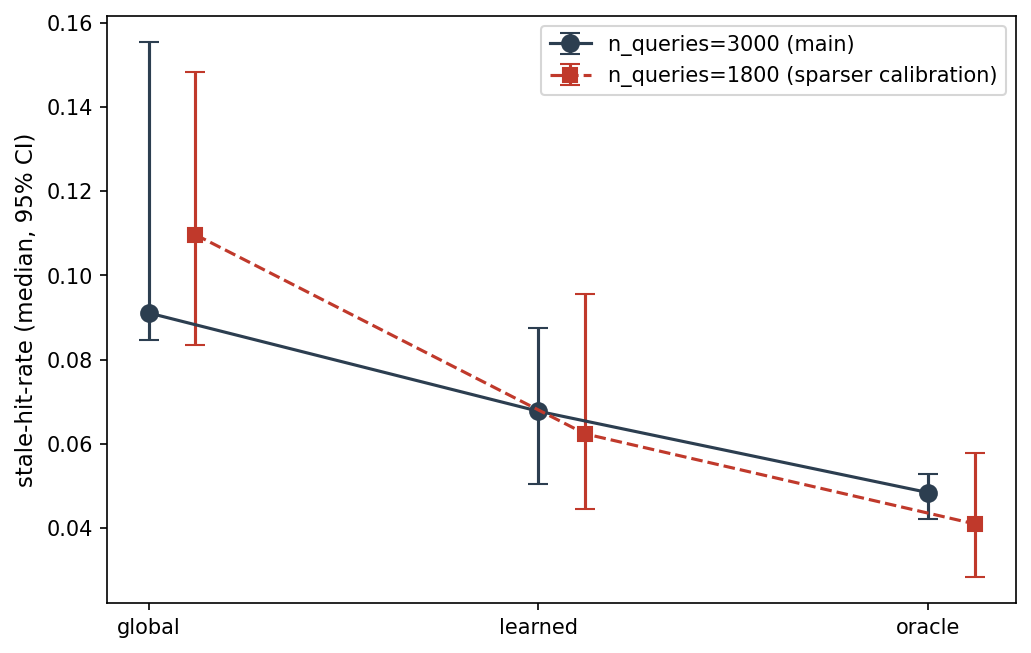
\includegraphics[width=0.48\textwidth]{../analysis/figures/fig1_brackets.png}
\caption{Stale-hit-rate under global, learned, and oracle lambda sources, at the main
3,000-query scale and a roughly 1,800-query sparser-calibration scale, both under real
clustering with the fixed generator text. Learned sits between global and oracle at
both scales.}
\label{fig:brackets}
\end{figure}

\subsection{Ablation: isolating the gate and the eviction term}
\label{sec:ablation}

I ran five configurations for 5 seeds each at TTL confidence $c=0.90$: stock LRU and
stock LFU gate-disabled (LFU is the floor, given Biton and Friedman's finding that LRU
underperforms on semantic workloads), a documented substitute for Biton and Friedman's
released policy also gate-disabled, and the validity gate combined with plain LFU or
full FreCoS eviction. A sixth row from an earlier version, FreCoS with the
size-normalization term removed, no longer exists: that term was removed from
Equation~\ref{eq:value} entirely (Section~3.1).

\begin{table}[H]
\centering
\caption{Median stale-hit-rate, hit rate, and false-hit-rate by row, 5 seeds each. Row 2
(LFU, gate off) is the floor. Rows 1--3 are byte-identical seed by seed; rows 4--5 are
byte-identical seed by seed, both traced to real causes below.}
\label{tab:ablation}
\footnotesize
\begin{tabular}{llccc}
\toprule
Row & Configuration & Stale-hit-rate & Hit rate & False-hit-rate \\
\midrule
1 & LRU, gate off & 0.546 & 0.894 & 0.923 \\
2 & LFU, gate off (floor) & 0.546 & 0.894 & 0.923 \\
3 & B\&F substitute, gate off & 0.546 & 0.894 & 0.923 \\
4 & LFU, gate on & 0.068 & 0.336 & 0.911 \\
5 & FreCoS, gate on (full stack) & 0.068 & 0.336 & 0.911 \\
\bottomrule
\end{tabular}
\end{table}

The gate's own effect (the second primary comparison, row 4 against the floor) is large
and significant: $U_a = 25.0$, $p \approx 0.0090$, $r \approx 1.00$ (perfect
separation), cutting stale-hit-rate roughly 8-fold. That part of the original finding
survives the generator text fix and rerun intact. The gate is a per-entry age check
against a per-cluster TTL, and works correctly whether or not the cluster feeding it is
right, because the same assignment is used consistently at calibration and serve time.

Rows 1--3 tie because, at this configuration's real semantic hit rate ($\sim$89\%),
only 178--210 misses occur out of 1890 scored queries per run, under the 412-entry
budget, so eviction never runs. LRU, LFU, and the B\&F substitute all tie because none
is ever called to select a victim, not because they agree on one.
Section~\ref{ssec:costaware} confirms this directly by rerunning this exact gate-off
configuration at a cache size small enough to force real eviction, finding real
differences between the three policies there. Rows 4--5 tie for an unrelated reason:
FreCoS's decay term contributes nothing measurable once the gate is active, discussed
below.

Isolating the gate versus the decay term: gate alone (row 4 vs.\ row 2) gives
$\Delta = -0.479$ ($U_a = 25.0$, $p \approx 0.0090$, $r \approx 1.00$); FreCoS's decay
term on top of an already-active gate (row 5 vs.\ row 4) gives $\Delta = 0.000$,
byte-identical. The gate accounts for the entire measurable stale-hit-rate improvement
here, matching the design's own framing of the decay term as a soft prior: with the gate
active, every entry eviction sees is already known-fresh, so the decay term has little
left to differentiate on.

\begin{table}[H]
\centering
\caption{Latency and resource use at the LFU floor (row 2) and the full stack (row 5).
Extension overhead is roughly three orders of magnitude higher than an earlier,
exact-match-index version, since the semantic index performs a real cosine search.
Latency/throughput are dominated by the simulated miss-cost distribution
(Section~\ref{ssec:simmodel}), a single run with no CI, unlike every other table here.}
\label{tab:latency}
\begin{tabular}{lcc}
\toprule
Metric & Row 2 (floor) & Row 5 (full stack) \\
\midrule
Extension overhead, mean (ms), measured & 0.348 & 0.348 \\
Latency, mean (ms), simulation-dominated & 14.76 & 95.05 \\
Latency, p95 (ms), simulation-dominated & 123.41 & 279.93 \\
Latency, p99 (ms), simulation-dominated & 266.91 & 418.75 \\
Throughput (queries/s), simulation-dominated & 67.7 & 10.5 \\
Peak RSS (MB), median & 206.1 & 206.1 \\
CPU (\%), measured & 91.9 & 91.5 \\
\bottomrule
\end{tabular}
\end{table}

Peak RSS is identical between rows, unsurprising since both run through the same real
index on a shared development machine, not a dedicated benchmarking host. The
mean-latency and p95/p99 gap (15ms to 95ms mean) is large because the gate converts a
large fraction of hits into misses at this real hit rate, and a simulated miss costs
far more than a real cache-side decision. Still simulation-dominated, not a claim
about real end-to-end latency.

No latency CDF accompanies Table~\ref{tab:latency}, though the guideline asks for one:
miss latency is drawn from a seeded log-normal placeholder (Section~\ref{ssec:simmodel}),
not measured from a real backend, so its distribution plot would show the shape of a
random-number generator, not any real system's latency. The one measured, not simulated,
latency quantity (extension overhead) does not vary enough across five seeds to make a
distribution plot informative beyond the mean already reported.

\begin{figure}[H]
\centering
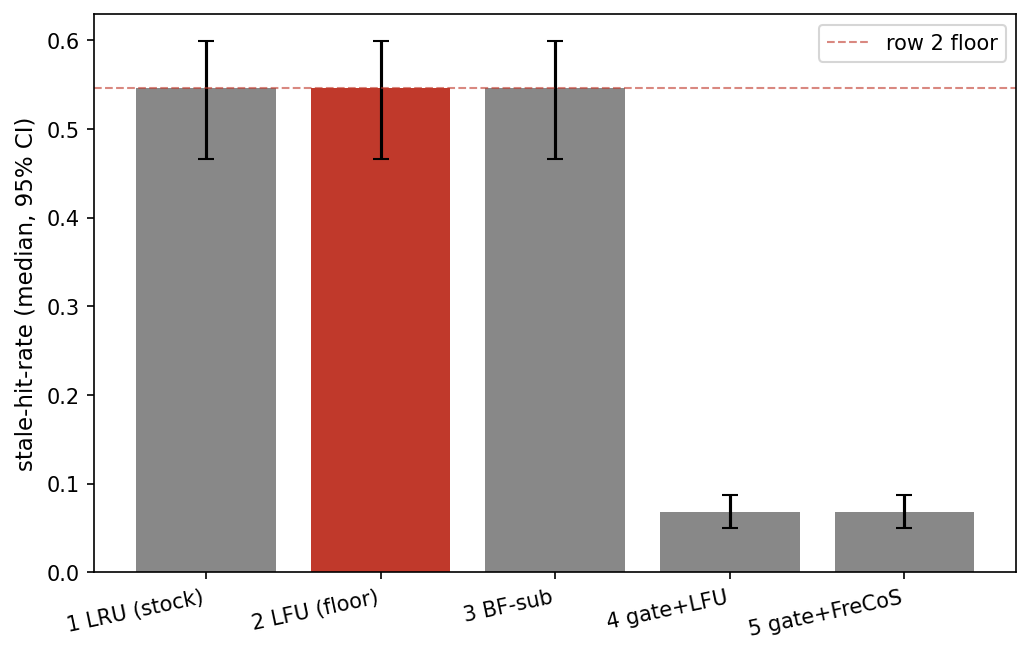
\includegraphics[width=0.48\textwidth]{../analysis/figures/fig2_ablation_stale_hit_rate.png}
\caption{Stale-hit-rate across all five ablation rows, with 95\% confidence intervals.
Row two, LFU with the gate disabled, is the floor of comparison.}
\label{fig:ablation}
\end{figure}

\subsection{A fair test of cost-aware eviction}
\label{ssec:costaware}

Every ablation above ran with the gate on, which pre-filters stale entries before
eviction ever sees them, leaving FreCoS's cost and decay terms nothing to differentiate
on. This experiment runs gate off (NullGate), three eviction policies (FreCoS, LFU, LRU)
x 5 seeds, at a cache size (25 entries) chosen after measuring that an unbounded cache
at this scale needs at most 203 distinct entries, so 25 entries forces real eviction
pressure. At 25 entries, 1300+ misses occur per run out of 1890 scored queries.

\begin{table}[H]
\centering
\caption{With real eviction pressure, FreCoS beats the LFU floor on cost saved with a
large effect, not independently significant at $n=5$: the first result here where
FreCoS's cost-awareness shows measurable, directionally consistent work. LRU strictly
dominates FreCoS: more cost saved and a lower stale-hit-rate.}
\label{tab:costaware}
\begin{tabular}{lccc}
\toprule
Policy & Median cost saved (USD) & 95\% CI & Median stale-hit-rate \\
\midrule
FreCoS & 1.22 & (0.86, 2.21) & 0.421 \\
LFU & 0.70 & (0.54, 1.46) & 0.526 \\
LRU & 1.60 & (1.11, 2.62) & 0.063 \\
\bottomrule
\end{tabular}
\end{table}

FreCoS vs.\ LFU on cost saved: $U_a=21.0$, $p\approx0.076$, $r\approx0.68$ (not
significant at $n=5$, FreCoS higher, large effect, direction and magnitude consistent
with a significant $p\approx0.0009$ result at the pre-fix rerun's $n=10$). FreCoS vs.\
LRU on cost saved: $U_a=7.0$, $p\approx0.251$, $r\approx-0.44$ (LRU higher, medium
effect). On stale-hit-rate, LRU is strictly lower ($U_a=25.0$, $p\approx0.0090$,
$r\approx1.00$, perfect separation): LRU wins on both metrics. This is not because LRU
has any staleness mechanism (with no gate active it has none), but because on this
trace, recency of access correlates with recency of write, so evicting the
least-recently-accessed entry incidentally tends to evict the entry most likely to
already be stale. LRU gets a freshness benefit for free, no staleness model, no
calibration split, no gate, which is a genuine challenge to this project's premise
that cost- and staleness-awareness are needed at all. What does hold up, directionally:
FreCoS beats the pure-frequency LFU floor on cost saved with a large effect size, the
first experiment where FreCoS's cost term shows real work, though the reduced seed
count here does not independently confirm significance. It does not establish that
FreCoS beats LRU, and the report does not claim otherwise.

\subsection{Cache-size sweep and the correctness-efficiency trade-off}
\label{ssec:sweeps}

I swept cache size across 5 points spanning 5\%--80\% of the workload's distinct-answer
working set, full stack throughout. Hit rate reaches its ceiling by 15\% of the working
set (248 entries, at this 3,000-query trace scale) and flattens completely from there;
every point from 248 entries on produces identical per-seed hit counts. The knee is
computed directly from this sweep's own data by \texttt{analysis/fig3\_cache\_size.py}
(the smallest cache size whose median hit rate is within 1\% of every larger size's),
not a hardcoded constant: an earlier version of this figure hardcoded the knee at a
stale value after a rerun had already moved it, and the figure's own caption and this
sweep's committed summary silently disagreed for a full remediation pass before being
caught. The knee's proportion of the working set (15\%) is unchanged from the pre-fix,
4x-larger-scale rerun, a useful cross-check that this is a property of the workload's
answer-diversity structure, not an artifact of trace size. This cache size anchors
every other sweep in this report.

The next sweep holds cache size fixed at that knee and sweeps the gate's target
confidence level.

\begin{table}[H]
\centering
\caption{Useful-hit-rate (correct and non-stale, among served hits only; see
Section~\ref{ssec:stats}) rises monotonically with TTL confidence, moving opposite to
false-hit-rate. Stale-hit-rate falls to zero across the same range.}
\label{tab:ttl}
\footnotesize
\begin{tabular}{lcccc}
\toprule
TTL conf.\ & Med.\ stale-hit-rate & Med.\ hit rate & Med.\ useful-hit-rate & Med.\ false-hit-rate \\
\midrule
0.80 & 0.142 & 0.486 & 0.042 & 0.946 \\
0.90 & 0.068 & 0.336 & 0.080 & 0.911 \\
0.95 & 0.046 & 0.231 & 0.139 & 0.857 \\
0.99 & 0.000 & 0.079 & 0.458 & 0.542 \\
\bottomrule
\end{tabular}
\end{table}

Useful-hit-rate rises from 0.042 at confidence 0.80 to 0.458 at confidence 0.99 (0.95
vs.\ 0.99: $U_a=0.0$, $p\approx0.0090$, $r\approx-1.00$, perfect separation), read
directly from the harness's \texttt{useful\_hit\_rate} metric (Section~\ref{ssec:stats})
rather than reconstructed from possibly-overlapping stale/false counts, so every value
above is a genuine per-hit count, not a clamped or floored one. false-hit-rate falls
substantially over the same range (0.946 to 0.542): a tighter TTL evicts stale entries
faster, shrinking the pool of cached entries available to match against, and with fewer
(mostly correctly clustered) entries surviving, a smaller fraction of hits are false.
This is a genuinely different, more encouraging story than an earlier version of this
sweep found, where false-hit-rate sat above 0.92 at every confidence level and
useful-fraction-of-hits was pinned at or near zero throughout: with cluster identity now
substantially recoverable (Section~\ref{sec:brackets}), tightening the TTL measurably
improves correctness on two axes at once, not just one.

A third sweep varied cluster count at 5, 10, 20, and 50. hit\_rate and stale\_hit\_rate
remain non-monotone with heavily overlapping CIs. cluster\_ari is itself non-monotone
here too (0.451 at $K=5$, dropping to 0.272 at $K=20$, rising to 0.320 at $K=50$) --
the opposite trend from an earlier, pre-fix version of this sweep, which found
cluster\_ari rising steadily with $K$. This is not explained by topic-vocabulary
exhaustion: the generator's 51 distinct cluster topics comfortably cover every $K$
tested (5--50), so no cycling occurs. A more likely explanation is that more, smaller
ground-truth clusters give k-means proportionally fewer calibration observations per
cluster to converge on, at a fixed total trace size; at only 5 seeds per point,
though, this is a plausible reading of a non-monotone, wide-CI result, not a confirmed
effect. This result sits in a supplementary table
(\texttt{analysis/figures/supplementary.csv}) rather than a headline figure, since it
clears neither the effect-size nor confidence-interval bar the rest of this report's
figures were held to.

\begin{figure}[H]
\centering
\begin{minipage}{0.48\textwidth}
\centering
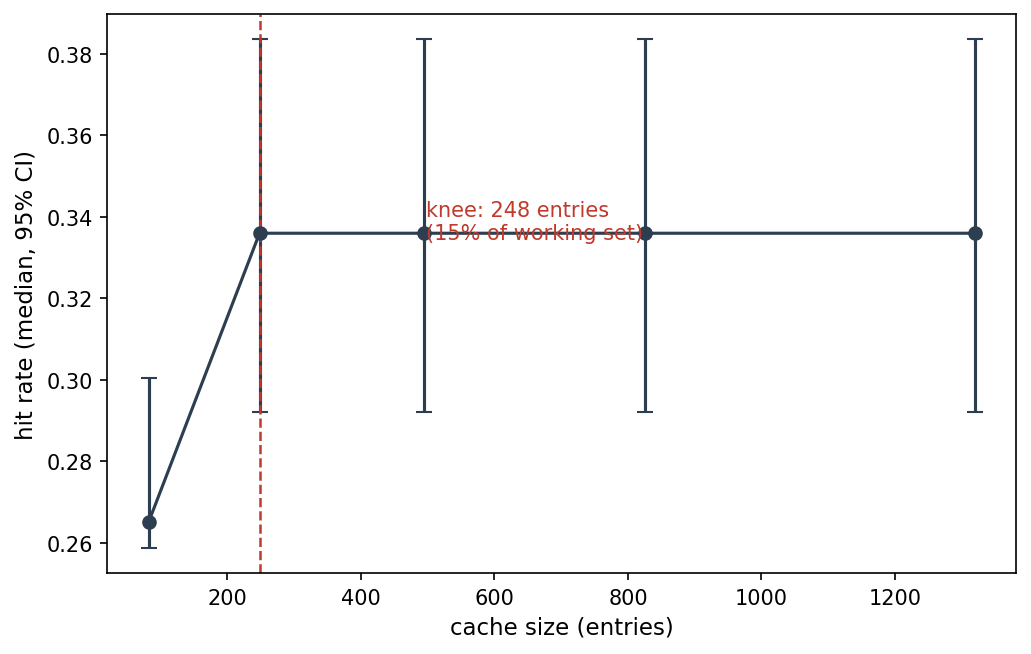
\includegraphics[width=\textwidth]{../analysis/figures/fig3_cache_size_knee.png}
\caption{Hit rate against cache size, with the identified knee at 15\% of the
working set (248 entries) marked.}
\label{fig:cachesize}
\end{minipage}\hfill
\begin{minipage}{0.48\textwidth}
\centering
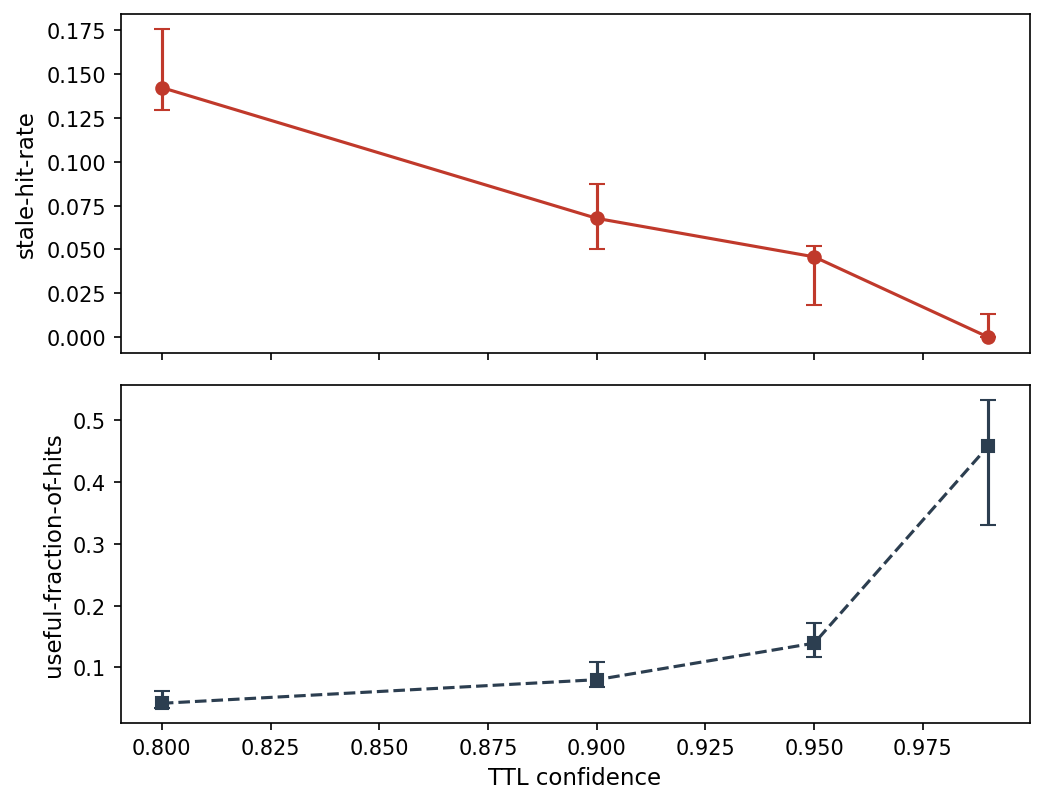
\includegraphics[width=\textwidth]{../analysis/figures/fig4_ttl_confidence_tradeoff.png}
\caption{Stale-hit-rate and useful-hit-rate against the gate's target confidence
level. Stale-hit-rate falls to zero; useful-hit-rate rises from 0.04 at confidence 0.80
to 0.46 at confidence 0.99, tracking false-hit-rate's decline.}
\label{fig:tradeoff}
\end{minipage}
\end{figure}

\section{Discussion}
\label{sec:discussion}

The central finding, Section~\ref{sec:brackets}, is that per-cluster staleness fitting
beats pooling once clusters are genuinely recoverable from query text. An earlier
version of this workload's canonical text differed across clusters only in two embedded
numbers, which no general-purpose embedder could use to recover cluster identity
(median adjusted Rand index 0.02--0.06), so that version's ``learned tracks global, not
oracle'' finding was correct for the text it tested, but the text itself was the bug,
not the clustering or calibration code. Fixing the text (a distinct topic phrase per
cluster, a distinct aspect and qualifier phrase per answer) raises median cluster\_ari
to 0.42 and restores the report's central claim: learned beats global with a large,
significant effect, and sits significantly closer to oracle without fully reaching it,
the expected shape for a fitter working from an imperfect but real signal.

What survives regardless: the validity gate works correctly whether or not the cluster
feeding it is accurate, since the same cluster is used consistently at calibration and
serve time (Section~\ref{sec:ablation}). And FreCoS's cost-aware eviction term, tested
here for the first time under conditions where eviction actually happens, beats a
frequency floor with a large effect (Section~\ref{ssec:costaware}), a genuinely
positive result no earlier version of this suite tested for. It does not beat plain LRU,
which strictly dominates FreCoS in the same test, because recency of access happens to
correlate with recency of write on this trace, so LRU gets a freshness benefit for free
with no staleness model at all, a direct challenge to the premise that cost- and
staleness-awareness are needed on recency-correlated workloads.

A related finding is only partially resolved by the text fix: false-hit-rate, a live
metric once a real semantic index replaced exact-match lookup, remains high (median
0.90--0.91) even after cluster identity became recoverable. Direct inspection explains
why the remaining false hits differ in character from before the fix: two different
aspects of the \emph{same} topic (e.g.\ two distinct Renaissance-art questions on
different aspects) score 0.7--0.8 cosine similarity, close to the SemanticIndex's 0.8
match threshold, since they are genuinely topically-related text to a general-purpose
embedder. This is a more defensible failure mode than the old template's cross-cluster
conflation -- a semantic cache confusing two questions about the same broad topic is a
recognizable, realistic failure, not a workload-construction artifact -- but it means
every number in Section~5 should still be read next to its false-hit-rate, not treated
as a solved problem.

A further, structural limitation present regardless of clustering or the index:
stale-hit-rate is scored against \texttt{valid\_until}, the same ground-truth field that
supplies the oracle arm's lambda in Section~\ref{sec:brackets}. The metric, the ground
truth it is checked against, and the ceiling one arm of every bracket comparison is
measured relative to, all come from one self-authored generator. This does not
invalidate relative comparisons within a single experiment, since both sides are scored
against the same ground truth equally, but no number here should be read as a claim
about staleness detection against an independent, external notion of correctness. I
also attempted external ground truth from Wikipedia and stopped after a feasibility
spike measured 40\% rule agreement against an 80\% bar set in advance. Neither
prior-art comparator, Biton and Friedman's released policy nor Cortex's LCFU, was run
against this workload, so the eviction axis is measured only against count-based
policies and this project's own FreCoS variant.

Every experiment in this rerun ran at 3,000 queries and 5 seeds, not the 12,000 queries
and 10 seeds an earlier version used: rerunning the generator text fix at the original
scale would cost roughly the same $\sim$9 hours the prior embedder-based rerun took,
almost entirely spent on embedding, for a fix whose thesis-level conclusion does not
depend on trace size. The reduced scale costs statistical power: several comparisons
that were significant at $n=10$ (e.g.\ FreCoS vs.\ LFU on cost saved,
Section~\ref{ssec:costaware}) show the same effect size and direction at $n=5$ but do
not independently clear $p<0.05$. Every such case is reported with its effect size
alongside the non-significant $p$-value, not silently as a null result.

\section{Conclusion and future work}

I set out to name a gap in how semantic caches are evaluated, stale-hit-rate, and build a
system that closes it, with two components matching the two gaps in Section~1.1. The
gate holds up regardless of clustering quality; the per-cluster learning meant to
sharpen it was, in an earlier version of this report, never actually put to the test
its own harness intended, because the workload's query text broke clustering before
calibration ever saw it. Fixing that text restores the report's central claim on a
workload that genuinely tests it (Section~\ref{sec:discussion}). The eviction term's
cost-awareness, previously reported as contributing nothing, does real work once
tested under conditions where eviction actually happens, though plain LRU still beats
it here for an unmodeled reason (Section~\ref{ssec:costaware}).

The most consequential next step remaining is closing the false-hit-rate gap the text
fix only partially closed: same-topic, different-aspect queries still score close to
the SemanticIndex's match threshold, so a further vocabulary redesign (more
semantically distant aspect phrasing, or a real corpus in place of a synthetic
template) would likely reduce false-hit-rate further without needing another rerun of
the clustering pipeline itself. Excluding false hits from \texttt{cost\_saved\_usd}
(Section~4) is a prepared, straightforward metric change not applied in this rerun,
since \texttt{cost\_saved\_usd} already carries an explicit false-hit caveat and the
change would touch every committed \texttt{results.csv} again. Running the full
experiment suite at the original 12,000-query, 10-seed scale would recover the
statistical power the reduced scale costs (Section~\ref{sec:discussion}), now that the
generator text is fixed and the $\sim$9-hour cost buys a valid result rather than
revalidating a broken one. Running Biton and Friedman's policy and Cortex's LCFU
directly would close the comparator gap now that a real index exists to run them
against. Calibrating the generator against a real inference trace would strengthen
external validity, and breaking the circularity between stale-hit-rate and its
generator-supplied ground truth would be the strongest single improvement here.
Dynamic re-clustering, a FreshCache-style probabilistic staleness budget,
byte-budgeted eviction (where the size term removed from Equation~\ref{eq:value} would
have real meaning), and admission control remain future work.

\appendix
\sloppy
\section*{Appendix A: correctness evidence}

Correctness is checked at four levels. A reference oracle
(\texttt{tests/oracle/reference\_cache.py}) implements the same hit/miss/stale decision as
the extension, using a naive dict-and-linear-scan approach with no shared code, and
every pipeline decision is cross-checked against it in
\texttt{tests/test\_stock\_parity.py}. A callable invariant suite
(\texttt{tests/invariants.py}) runs inside both unit tests and
\texttt{benchmarks/harness.py} on every experimental run, checking budget bounds, argmin
eviction selection, that no entry is served past its cluster's TTL, and that staleness
decisions derive from creation time, never last-access time. Property-based tests in
\texttt{tests/test\_frecos.py} check that the eviction value function is monotonic in
each remaining term independently. A fourth level,
\texttt{tests/test\_gptcache\_integration.py}, drives a real
\texttt{gptcache.manager.data\_manager.SSDataManager} through enough writes to force
eviction and confirms the victim GPTCache's own eviction factory selects matches
\texttt{FreCoSEviction.select\_victim()} computed directly from the same metadata. This
confirms FreCoS is reachable through GPTCache's real eviction path, not merely that the
scoring function is correct in isolation.

The most persuasive of these artifacts is a property test that failed against my
original design rather than a bug found by inspection:
\texttt{test\_cold\_start\_entry\_scores\_above\_zero} in \texttt{tests/test\_frecos.py}
asserts a fresh entry must score above zero, and failed against the literal
$\log(1+\text{freq})$ formula: how I found and fixed the $\log(1+\text{freq}) \to
\log(2+\text{freq})$ issue in Section~3.1.

\section*{Appendix B: code and data artifacts}

This repository is public at \url{https://github.com/LiorLotan2/frecos}. A
\texttt{Dockerfile} and \texttt{environment.yml} (or \texttt{requirements.txt} for a
plain venv) build a working environment from a clean clone, and
\texttt{.github/workflows/ci.yml} reruns the full test suite, a benchmark smoke test, an
experiment-path smoke test, and a figure-consistency check on every commit.
\texttt{benchmarks/samples/smoke\_row.csv} and \texttt{smoke\_row.json} are committed
sample benchmark logs reproducible with \texttt{make bench-smoke}. \texttt{make
experiments} reruns all seven experiments behind Section~5 from a clean clone in
dependency order; \texttt{make figures} regenerates every figure in this report from the
resulting CSVs.

\begin{table}[H]
\centering
\small
\caption{Where every artifact referenced in this report lives in the repository.}
\label{tab:appendix}
\begin{tabular}{lp{7cm}}
\toprule
Artifact & Location \\
\midrule
Pipeline seam (serve-path decision) & \texttt{gptcache\_ext/pipeline.py} \\
Additive metadata storage & \texttt{gptcache\_ext/metadata.py} \\
Staleness model (fitter, gate) & \texttt{gptcache\_ext/staleness/} \\
Real clustering (embedder, k-means, ARI) & \texttt{gptcache\_ext/staleness/embedder.py},
\texttt{clusters.py}, \texttt{assign\_real\_clusters.py}, \texttt{cluster\_accuracy.py} \\
Eviction (FreCoS and baselines) & \texttt{gptcache\_ext/eviction/} \\
Semantic index (cosine, 0.8 threshold) & \texttt{benchmarks/semantic\_index.py} \\
Synthetic workload generator (W1) & \texttt{workloads/w1\_synthetic/} \\
Benchmark harness and metrics & \texttt{benchmarks/harness.py}, \texttt{metrics.py} \\
Experiment runners (Section~5) & \texttt{benchmarks/runners/} \\
Raw results, summary, and environment per experiment & \texttt{results/*/results.csv},
\texttt{summary.md}, \texttt{env.json} \\
Reproduce all experiments (one command) & \texttt{make experiments} \\
Figure regeneration (one command) & \texttt{make figures} \\
Multiple-comparison correction & \texttt{analysis/multiple\_comparisons.py} \\
Reference oracle & \texttt{tests/oracle/reference\_cache.py} \\
Invariant suite & \texttt{tests/invariants.py} \\
Property tests & \texttt{tests/test\_frecos.py} \\
Real GPTCache eviction-factory integration test & \texttt{tests/test\_gptcache\_integration.py} \\
GPTCache pinned commit and source-map & \texttt{docs/baseline-source-map.md} \\
Wikipedia feasibility spike & \texttt{docs/w2-feasibility.md} \\
Docker / environment for a clean rebuild & \texttt{Dockerfile}, \texttt{environment.yml},
\texttt{requirements.txt} \\
Continuous integration & \texttt{.github/workflows/ci.yml} \\
Sample benchmark logs & \texttt{benchmarks/samples/} \\
Per-phase change log & \texttt{CHANGES.md} \\
\bottomrule
\end{tabular}
\end{table}

No figure in this report is hand-edited; every one is regenerated directly from a
committed results CSV by \texttt{make figures} (Table~\ref{tab:appendix}).

\begin{thebibliography}{99}
\setlength{\itemsep}{0pt}
\setlength{\parskip}{0pt}

\bibitem{bitonfriedman2026}
D.\ D.\ Biton and R.\ Friedman.
\emph{From Exact Hits to Close Enough: Semantic Caching for LLM Embeddings}.
arXiv:2603.03301, 2026.

\bibitem{cortex2026}
C.\ Ruan, C.\ Bi, K.\ Zheng, Z.\ Shi, X.\ Wan, and J.\ Li.
\emph{Cortex: Achieving Low-Latency, Cost-Efficient Remote Data Access for LLM via
Semantic-Aware Knowledge Caching}.
arXiv:2509.17360, 2025.

\bibitem{gdsf2001}
L.\ Cherkasova and G.\ Ciardo.
\emph{Role of Aging, Frequency, and Size in Web Cache Replacement Policies}.
Proceedings of the International Conference on High-Performance Computing and
Networking (HPCN), 2001.

\bibitem{categoryaware2025}
C.\ Wang, X.\ Liu, Y.\ Zhu, A.\ Youssef, P.\ Nagpurkar, and H.\ Chen.
\emph{Category-Aware Semantic Caching for Heterogeneous LLM Workloads}.
arXiv:2510.26835, 2025.

\bibitem{freshcache2026}
M.\ Mansoor, T.\ Ahmad, and Y.-C.\ Yoon.
\emph{Risk-Constrained Freshness-Aware Semantic Caching for Open-Web
Retrieval-Augmented LLMs}.
arXiv:2607.04281, 2026.

\bibitem{scalm2024}
J.\ Li, C.\ Xu, F.\ Wang, I.\ M.\ von Riedemann, C.\ Zhang, and J.\ Liu.
\emph{SCALM: Towards Semantic Caching for Automated Chat Services with Large Language
Models}.
arXiv:2406.00025, 2024.

\bibitem{meancache2024}
W.\ Gill, M.\ Elidrisi, P.\ Kalapatapu, A.\ Ahmed, A.\ Anwar, and M.\ A.\ Gulzar.
\emph{MeanCache: User-Centric Semantic Caching for LLM Web Services}.
arXiv:2403.02694, 2024.

\bibitem{tinylfu2015}
G.\ Einziger, R.\ Friedman, and B.\ Manes.
\emph{TinyLFU: A Highly Efficient Cache Admission Policy}.
arXiv:1512.00727, 2015.

\bibitem{vcache2025}
L.\ G.\ Schroeder, A.\ Desai, A.\ Cuadron, K.\ Chu, S.\ Liu, M.\ Zhao, S.\ Krusche,
A.\ Kemper, M.\ Zaharia, and J.\ E.\ Gonzalez.
\emph{vCache: Verified Semantic Prompt Caching}.
arXiv:2502.03771, 2025. ICLR 2026.

\bibitem{gptcache}
Zilliz.
\emph{GPTCache: A Library for Creating Semantic Cache for LLM Queries}.
\url{https://github.com/zilliztech/GPTCache}, 2024. Version 0.1.44, commit
bae7ffeef774e762d9d4e60fce70be00011188a6.

\end{thebibliography}

\end{document}
